\chapter{Upsampling Layer (``Transposed Convolution")}
\subsection*{Learnable Upsampling}

\begin{figure}[h]
  \centering
  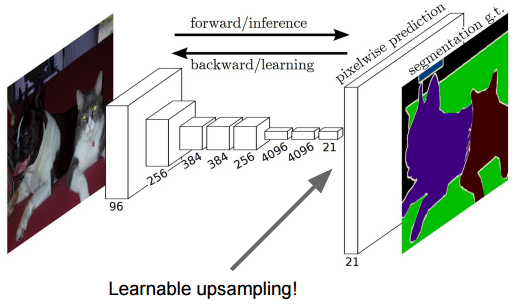
\includegraphics[width=0.5\textwidth]{Images/upsampling_layer/1.png}
  \caption{From the paper: ``Fully Convolutional Networks for Semantic Segmentation"}
\end{figure}



\subsection*{Transposed Convolution}
Transposed convolutions -- also called fractionally strided convolutions -- work by swapping the forward and backward passes of a convolution. One way to put it is to note that the kernel defines a convolution, but whether it’s a direct convolution or a transposed convolution is determined by how the forward and backward passes are computed.

The transposed convolution is implemented as the backward pass of a  corresponding non-transposed convolution. It can be thought of as dilating  the input (by adding ``stride - 1" zeros between adjacent input elements),  padding it with the needed number of zeros so it is not out. And then, apply the convolution with the filter flipped 180 degrees.

\begin{figure}[h]
  \centering
  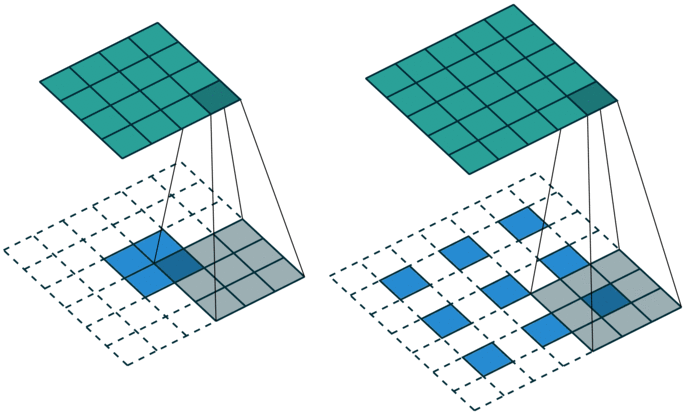
\includegraphics[width=0.4\textwidth]{Images/upsampling_layer/5.png}
  \caption{\textbf{Left}: Visually, for a transposed convolution with stride one and no padding, we just pad the original input (blue entries) with zeroes (white entries). \textbf{Right}: Stride two and padding, the transposed convolution would look like this
}
\end{figure}

\subsection*{Skip Connections}

\begin{figure}[h]
  \centering
  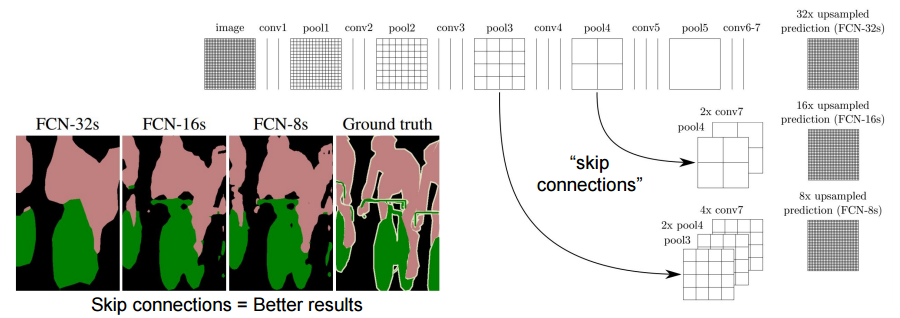
\includegraphics[width=0.8\textwidth]{Images/upsampling_layer/4.png}
  \caption{Skip Connections}
\end{figure}
